\chapter{Theory}
This section addresses necessary theory needed to understand the project.

\section{Word Embeddings}

\section{Recurrent Neural Networks}
Recurrent Neural Networks (RNNs) are a flavour of Artificial Neural Networks (ANNs) designed to work with sequential data~\cite{goodfellow2016deep}. While an ANN can be presented with sequential data as well, it lacks the capability of preserving a context throughout it. This is solved by RNNs by introducing dependencies on previous sequential steps through additional connections.
\begin{figure}[H]
  \centering
  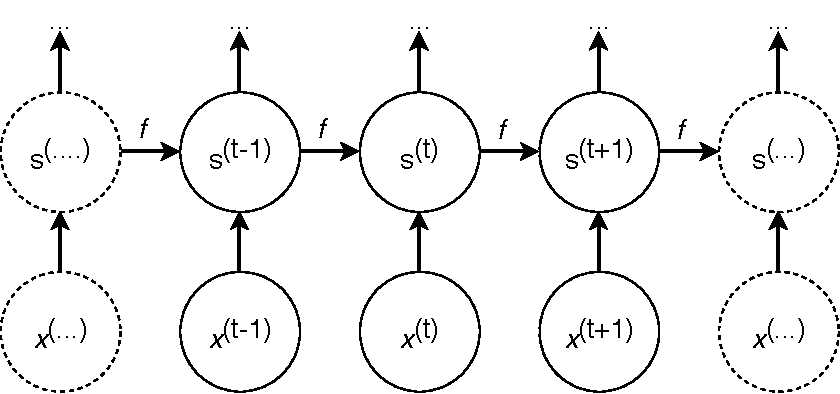
\includegraphics[width=0.8\textwidth]{graphics/rnn}
  \caption{An illustration of an RNN for input sequence $x$, where $h$ is the hidden unit activation functions and $f$ a function describing the relationship between two concurrent states~\cite{goodfellow2016deep}.}\label{fig:rnn}
\end{figure}
An illustration of an RNN can be seen in Figure~\ref{fig:rnn} which shows the context-preserving connections between states $s^{(t)}$. There are many ways to structure RNNs, depending on the problem at hand, but other structures are out of scope for this project.

Training of RNNs is done using the \textit{backpropagation} algorithm, which is an efficient way to perform gradient descent optimization of the networks weights. However, in the case of long-term dependencies the gradients tend to become vanishingly small (or in some rare cases tend towards infinity) which hinders training. One solution to this problem is to use so called \textit{gated RNNs}, more specifically Long Short-Term Memory Networks (LSTMs).

\subsection{Long Short-Term Memory Networks}
LSTMs are RNNs with a more complicated cell structure for the hidden units, which have shown to much better capture long-term dependencies than the simpler structure of standard hidden units~\cite{hochreiter1997long}. They work by containing an internal state which is regulated by the input.

